\documentclass[10pt]{beamer}
\usepackage{uglixbeamer,animate}
\subtitle{Chapitre 01}
\title{Récursivité}
\author{NSI2}
\begin{document}

\maketitle
\begin{frame}
\begin{center}

\includegraphics[width=3cm]{img/troll}
\end{center}\pause
\textit{Pour comprendre la récursivité, il faut d'abord comprendre la récursivité.}\\
\end{frame}




\section{Le formidable principe de la récursivité\\ (la forme)}




\begin{frame}{S'appeler et se terminer}
On dit qu'une fonction est \alert{récursive} lorsque dans sa définition on appelle (une ou plusieurs fois)
cette même fonction.\\\pause

Cela pose un problème : si la fonction ne cesse de s'appeler, comment
cela peut-il se terminer ?
\end{frame}




\begin{frame}[fragile]{Exemple 1}
La fonction suivante est incorrecte :
\begin{minted}{python}
def f():
    return f()
\end{minted}
\pause
l'appel \pythoninline{f()} provoque \textit{a priori} une boucle infinie.
\end{frame}




\begin{frame}[fragile]{Exemple 2}
\begin{minted}{python}
def f(n : int):
    return f(n-1)
\end{minted}
\pause
Quelle que soit la valeur de \pythoninline{x}, l'appel \pythoninline{f(x)} provoque également \textit{a priori} une boucle infinie :\\\pause
\pythoninline{f(10)} appelle \pythoninline{f(9)} qui appelle \pythoninline{f(8)} \textit{et c\ae tera}.
\end{frame}


\begin{frame}[fragile]{Nécessité d'une condition d'arrêt}
\begin{minted}{python}
def f(n : int) -> int:
    if n <= 0 :
        return 0
    else:
        return f(n - 1)
\end{minted}
\pause
\only<2>{
Cette fonction n'est pas très utile...
}

\only<3>{
Dans le corps de cette fonction, on distingue 2 cas :
\begin{enumerate}[\textbullet]
	\item 	le \alert{cas d'arrêt}, dans lequel \pythoninline{n <= 0} et la fonction renvoie zéro;\pause
	\item 	le \alert{cas récursif} dans lequel la fonction s'appelle elle-même.
\end{enumerate}
}

\only<4>{
Quel que soit l'entier \pythoninline{n} de départ (qu'on suppose grand), lorsqu'on évalue \pythoninline{f(n)} alors celle-ci évalue \pythoninline{f(n-1)} qui elle-même évalue \pythoninline{f(n-2)} \textit{et c\ae tera}.\\

Puisque les nombres \pythoninline{n-1}, \pythoninline{n-2}, \pythoninline{n-3}, $\ldots$ diminuent strictement, les appels récursifs \alert{vont finir par laisser place au cas d'arrêt} de sorte que \pythoninline{f(n)} est bien défini.}
\end{frame}


\begin{frame}[fragile]{\textit{Syntactic Sugar}}
\begin{center}

\includegraphics[width=6cm]{img/syntactic_sugar}
\end{center}
 « sucre syntaxique » d'un langage de programmation : ensemble des règles de syntaxe qui ont été ajoutées pour rendre le code plus facile à lire et à écrire.\pause
\begin{minted}{python}
def f(n : int) -> int:
    return 0 if n <= 0 else f(n - 1)
\end{minted}
\end{frame}




\begin{frame}[fragile]{Un premier exemple digne d'intérêt}
Soit $n\in\N$. \textit{Factorielle} $n$ est le produit de tous les entiers non-nuls inférieurs ou égaux à $n$, et se note $n!$.\pause
\begin{itemize}
	\item $1!=1$;\pause
	\item $2!=1\times2 = 2$;\pause
	\item $10!=1\times 2\times \ldots \times 10 = \np{3628800}$;\pause
	\item $0! = 1$ par convention.
\end{itemize}
\end{frame}


\begin{frame}[fragile]{À l'aide d'une boucle for}
\begin{minted}{python}
def factorielle( n : int) -> int:
    result = 1
    for i in range(1, n + 1):
        result *= i
    return result
\end{minted}
\pause
L'algorithme est dit \alert{itératif} car il utilise une boucle.
\end{frame}


\begin{frame}[fragile]{De manière récursive}
\begin{minted}[fontsize=\footnotesize]{pseudocode}
fonction factorielle(n : entier naturel) -> entier naturel
    si n = 0 alors
        renvoyer 1
    sinon
        renvoyer n * factorielle(n -1)
    fin si
\end{minted}

\pause
D'une certaine manière, c'est plus « élégant ».
\end{frame}



\begin{frame}{Pour s'entraîner}

\begin{alertblock}{Exercice}
\begin{enumerate}[\bfseries 1.]
	\item 	Programmer la fonction \mintinline[bgcolor=codebackground]{python}{factorielle} en \textsc{Python} de manière récursive, et tester cette fonction en vérifiant que  \mintinline[bgcolor=codebackground]{python}{factorielle(10)} renvoie bien \np{3628800}.
    \item   Mettre du \textit{Syntactic Sugar} là-dedans !
\end{enumerate}
\end{alertblock}
\end{frame}




\section{Formidable, mais pourquoi\\ (le fond)?}



\begin{frame}{Principe}
\begin{enumerate}[--]
	\item 	On veut écrire une fonction \pythoninline{f} qui résout un problème dépendant d'un entier naturel \pythoninline{n};\pause
	\item 	on examine le cas ou \pythoninline{n} vaut 0 (ou 1), correspondant à un problème très simple, que l'on sait résoudre;\pause
	\item 	on suppose que l'on sait résoudre le problème pour un entier \pythoninline{n-1}, à l'aide de la fonction \pythoninline{f}, on regarde alors les opérations à effectuer pour passer de ce problème au problème de taille \pythoninline{n};\pause
	\item 	on programme alors la fonction \pythoninline{f} de manière récursive.
\end{enumerate}
\end{frame}





\begin{frame}[fragile]{L'exemple des poignées de main}

Nous l'avons traité en activité préparatoire :

\begin{minted}{python}
def f(n : int) -> int
    return 0 if n == 0 else n - 1 + f(n - 1)
\end{minted}
\end{frame}



\begin{frame}{Un exemple de récursion double}
\begin{center}
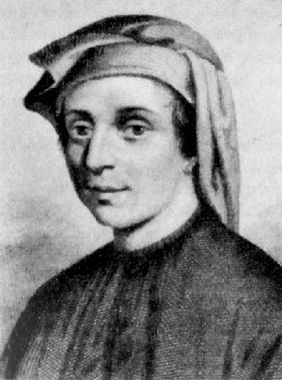
\includegraphics[width=2cm]{img/fibonacci}
\end{center}
La célèbre suite de Fibonacci, notée $F$, est définie ainsi :\pause
\begin{enumerate}[--]
	\item 	Ses deux premiers termes $F_0$ et $F_1$ valent 1;\pause
	\item 	On construit chaque terme suivant en faisant la somme des deux précédents.
\end{enumerate}
\end{frame}




\begin{frame}{Un exemple de récursion double}
De proche en proche, on calcule :\pause
\begin{enumerate}[--]
	\item $F_2=1+1=2$\pause
    \item  $F_3=2+1=3$\pause
    \item $F_4=3+2=5$\pause
    \item \textit{et c\ae tera}\pause
\end{enumerate}
Et plus généralement\pause
$$F_n=\begin{cases}
1 & \mbox{si } n=0\mbox{ ou }n=1\\
F_{n-1}+F_{n-2} &\mbox{sinon}
\end{cases}$$
\end{frame}
\begin{frame}[fragile]{Algorithme}
\begin{minted}[fontsize=\footnotesize]{pseudocode}
fonction fibonacci(n : entier naturel) -> entier naturel
    si n < 2 alors
        renvoyer 1
    sinon
        renvoyer fibonacci(n - 1) + fibonacci(n - 2)
    fin si
\end{minted}
\end{frame}




\begin{frame}{Pour s'entraîner}
\begin{alertblock}{Exercice}
Programmer la fonction  \mintinline[bgcolor=codebackground]{python}{fibonacci} en \textsc{Python} et vérifier que  \mintinline[bgcolor=codebackground]{python}{fibonacci(30)} vaut \np{1346269}.
\end{alertblock}
\end{frame}




\begin{frame}{Remarques}
\begin{enumerate}[--]
	\item La récursivité est un des concepts \textit{fondamentaux} de l'informatique.\\\pause
            On dit que c'est un \alert{paradigme de programmation}.\pause
    \item Certains algorithmes se programment naturellement de manière récursive.\pause
    \item Certaines \alert{structures de données} se définissent également de manière récursive.
\end{enumerate}
\end{frame}




\section{La \og magie\fg{} a un coût}




\begin{frame}{La pile d'appels}
Que se passe-t-il réellement en machine lorsqu'on évalue la fonction récursive \pythoninline{factorielle(3)} ?\\\pause

\textsc{Python} possède une \alert{pile} : c'est une structure de données simple, qui permet d'empiler et de dépiler des données un peu comme on empile des assiettes.\\  \pause

Lors de chaque appel récursif, une valeur est empilée en attendant le résultat de l'appel.
\end{frame}





\begin{frame}{}
\begin{center}
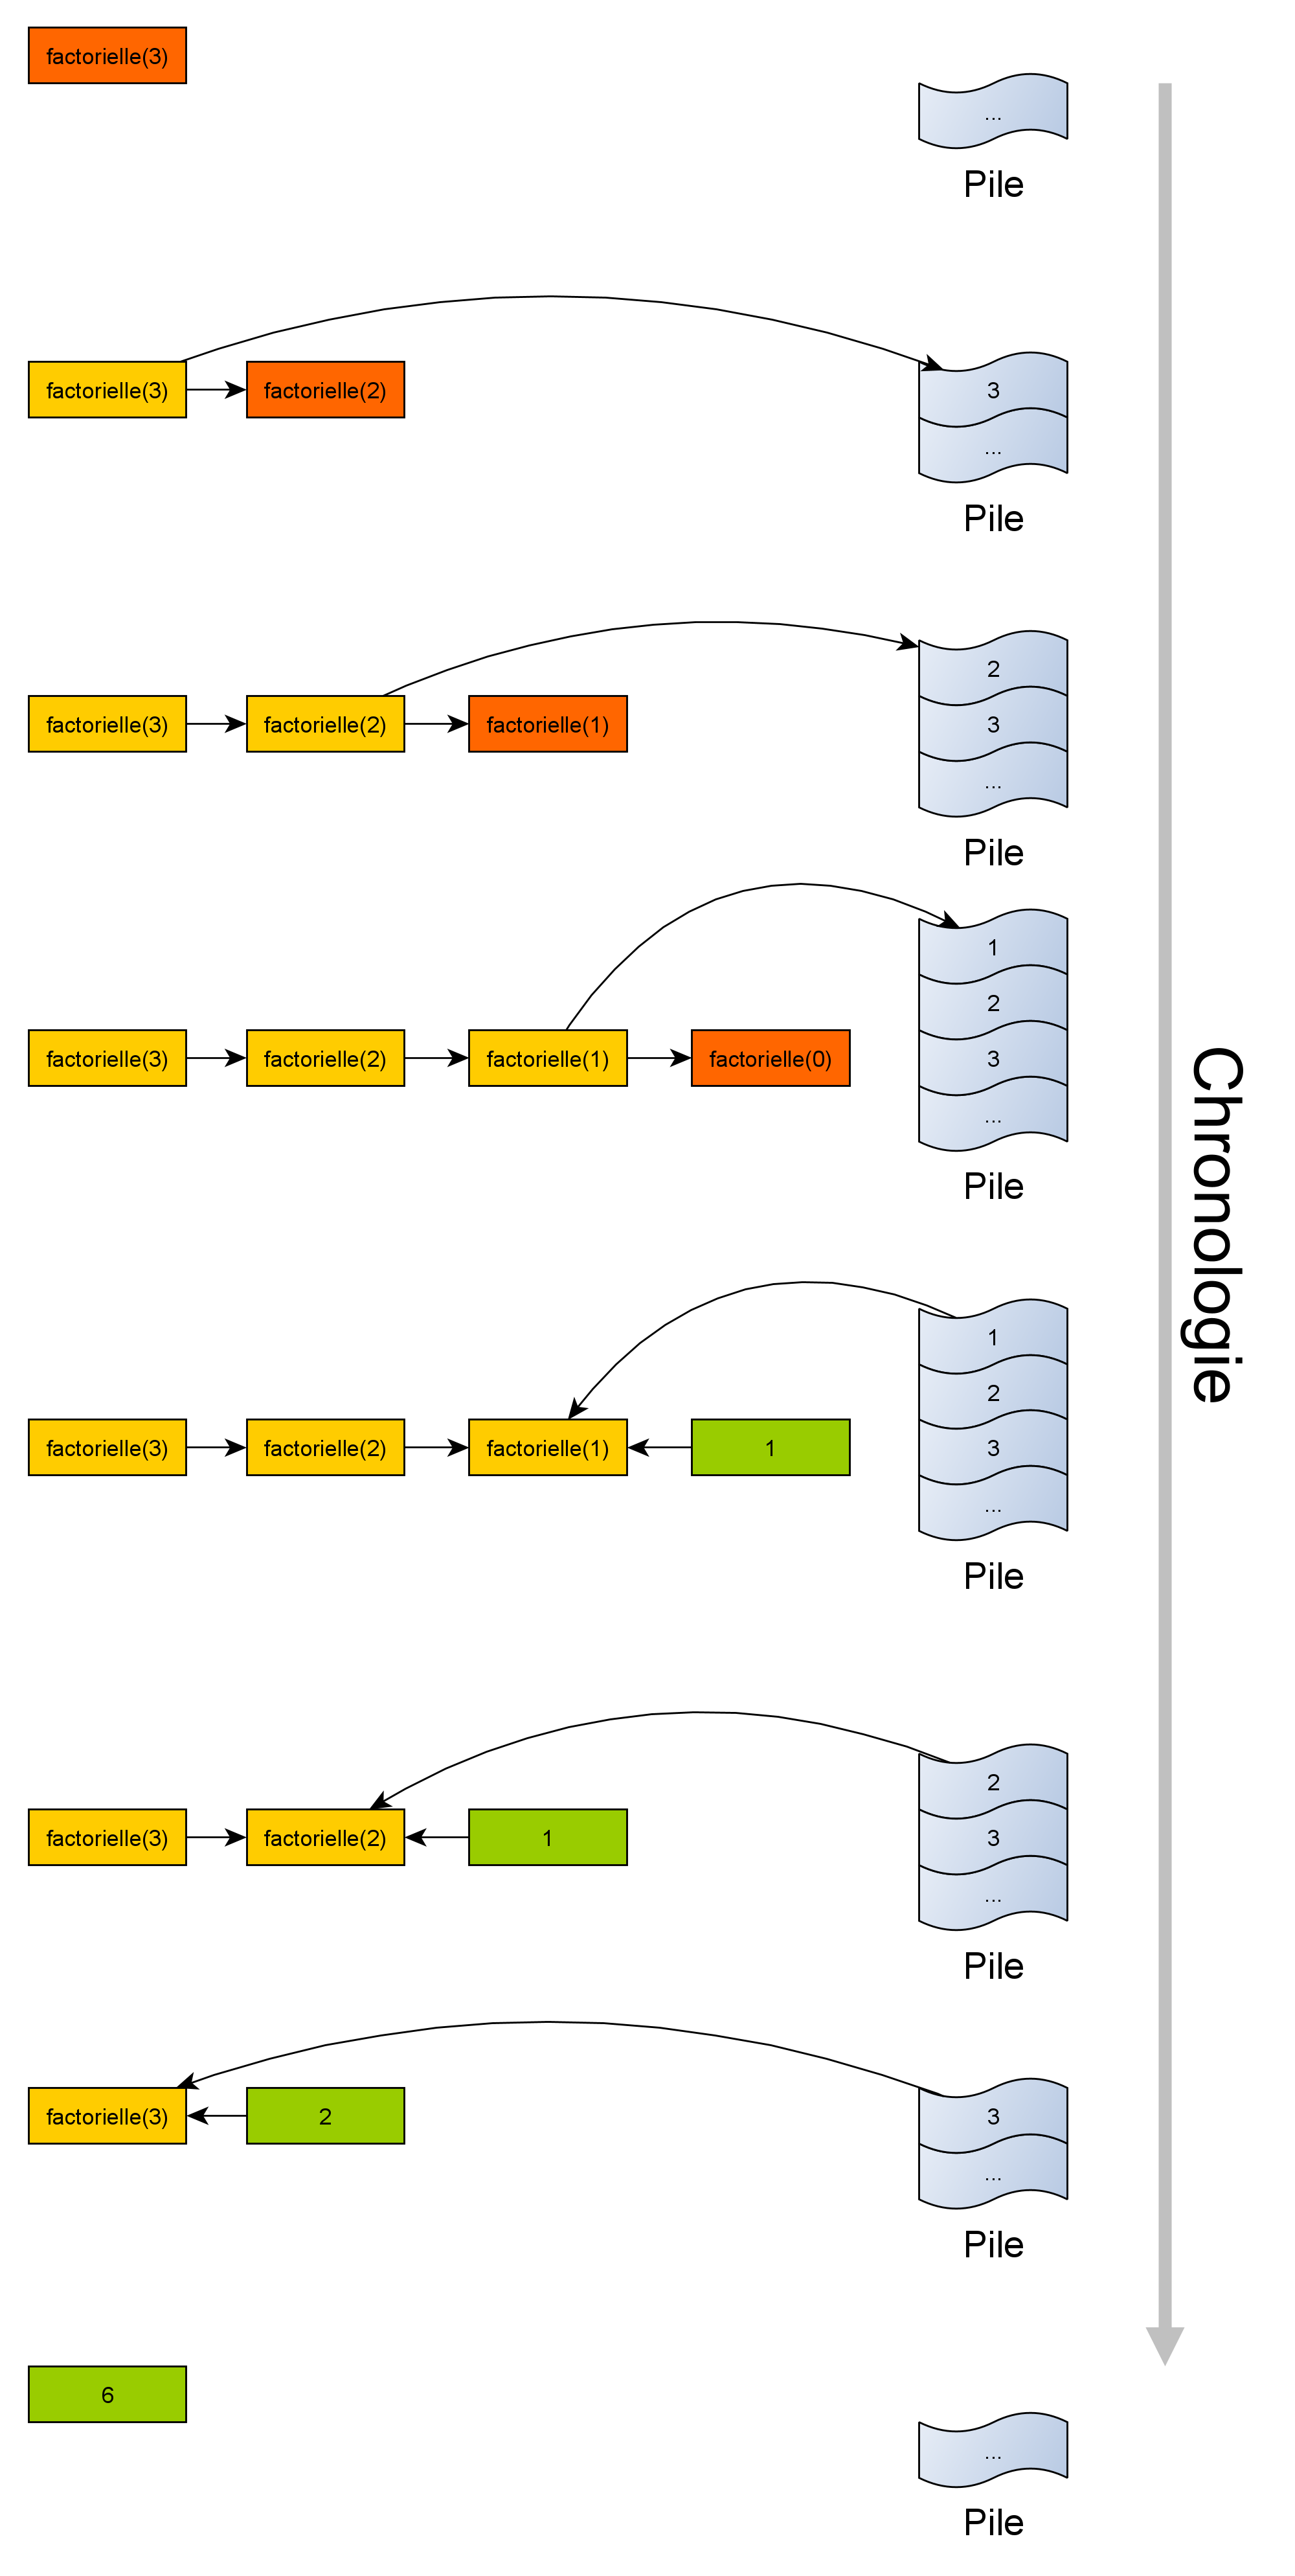
\includegraphics[width=4cm]{img/appels}
\end{center}
\end{frame}





\begin{frame}{Taille de la pile}
Lorsqu'il y a beaucoup d'appels récursifs \textit{imbriqués}, la taille de la pile augmente.\\\pause
Pour éviter qu'elle sature, \textsc{Python} fixe la limite des appels récursifs \textit{imbriqués} à 999. Dès que l'on dépasse cette limite on obtient un message d'erreur :\\\pause

\color{red} \texttt{\footnotesize RecursionError: maximum recursion depth exceeded in comparison}\color{black}\\
\end{frame}




\begin{frame}[fragile]{Fixer la taille de la pile}
\begin{minted}{python}
import sys

sys.setrecursionlimit(10_000)
\end{minted}

Pour aller jusqu'à \np{10000} appels récursifs au maximum (par exemple).
\end{frame}




\begin{frame}{Pour s'entraîner}
\begin{alertblock}{Exercice}
Reprendre la fonction récursive \mintinline[bgcolor=codebackground]{python}{fibonacci} et utiliser le site \link{http://pythontutor.com/visualize.html}{Python Tutor} pour visualiser la pile d'appels lors de l'évaluation de \mintinline[bgcolor=codebackground]{python}{fibonacci(5)}.\\

Quel commentaire peut-on faire ?
\end{alertblock}
\end{frame}
\end{document}
